\documentclass{ltjsarticle}
\usepackage{booktabs}
\usepackage{mathcomp}
\usepackage{array}
\usepackage{mathtools,amssymb}
\usepackage{siunitx}
\usepackage{multirow}
\usepackage{tabularx}
\usepackage{subcaption}
\usepackage{float}
\usepackage{kcctd-report}
\usepackage{listings,jvlisting}

\title{光情報通信に関する実験}
\adviser{荻原昭文}

\sdate{令和5年12月14日}
\edate{令和5年12月21日}
\fdate{令和5年12月26日}
\rdate{}

\grade{5}
\anumber{}
\gnumber{B}
\name{河合将暉}
\jname{岡田}
\comment{}
\begin{document}
\maketitle

\section{目的}
	LED,レーザ等による発光現象の測定やフォトダイオードによる光検出回路の作製実験
	を通じて光情報通信の原理を理解する.

\section{解説}
	\subsection{2分割フォトダイオード}
	\subsection{圧電効果と逆圧電効果}
		圧電効果とは,\cite{ref:圧電効果}によると,水晶や特定のセラミックなどに圧力を加えることで生じるひずみに応じて,
		電圧が発生する現象である.これは,固体結晶内部のイオン配置のずれが圧力を加えることで大きくなり,結晶の一端が
		プラスの電荷を帯び,もう一方にはマイナスの電荷が発生する電気分極という現象によって電圧が発生している。
		反対に,水晶やセラミックなどに電圧を加えると結晶が変形することを逆圧電効果という.
	\subsection{圧電セラミック素子}
		圧電効果を利用して電気を取り出したり,逆に電圧をかけることで振動を取り出す素子のことを圧電(ピエゾ)素子と呼ぶ.
		\cite{ref:圧電効果}より引用した圧電素子の構造を図\refeq{fig:圧電素子}に示す.
		\begin{figure}[H]
		\centering
		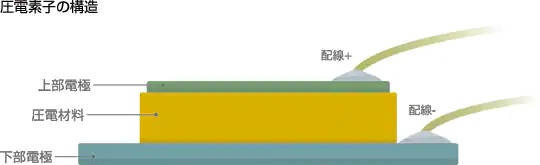
\includegraphics[width = 12cm]{figs/kl080302u.jpg}
		\caption{圧電素子の構造図}
		\label{fig:圧電素子}
		\end{figure}
\section{実験方法}
	\subsection{使用器具}
		本実験での使用器具を表\refeq{tab:used}に示す.
		\begin{table}[H]
		\begin{center}
		\caption{使用器具}
		\label{tab:used}
		\begin{tabular}{clllll} \toprule
		No&\multicolumn{1}{c}{機器名}&\multicolumn{1}{c}{企業名}&\multicolumn{1}{c}{型番}&\multicolumn{1}{c}{シリアルNo}&\multicolumn{1}{c}{備考}\\
		\hline
		1&DMM&sanwa&PC-5000&\\
		2&オシロスコープ&Tektronix&TBS 1052B&\\
		3&FG&A&D&AD-8623A&\\
		4&オペアンプ&&INA103&\\
		5&圧電セラミック素子&&&\\
		6&レーザダイオード&&&\\
		7&2分割フォトダイオード&&&\\
		8&各種回路素子&&&\\
		\bottomrule
		\end{tabular}
		\end{center}
		\end{table}

	\subsection{圧電セラミック素子への電圧印加による共振現象の測定}
		図にLDと差分増幅回路を用いた圧電セラミック素子への電圧印加による測定システムを示す.
		PZTの厚さdは電極板とPZTとを積層した厚さと電極板のみの厚さの差分から求められる.
		\begin{figure}[H]
		\centering
		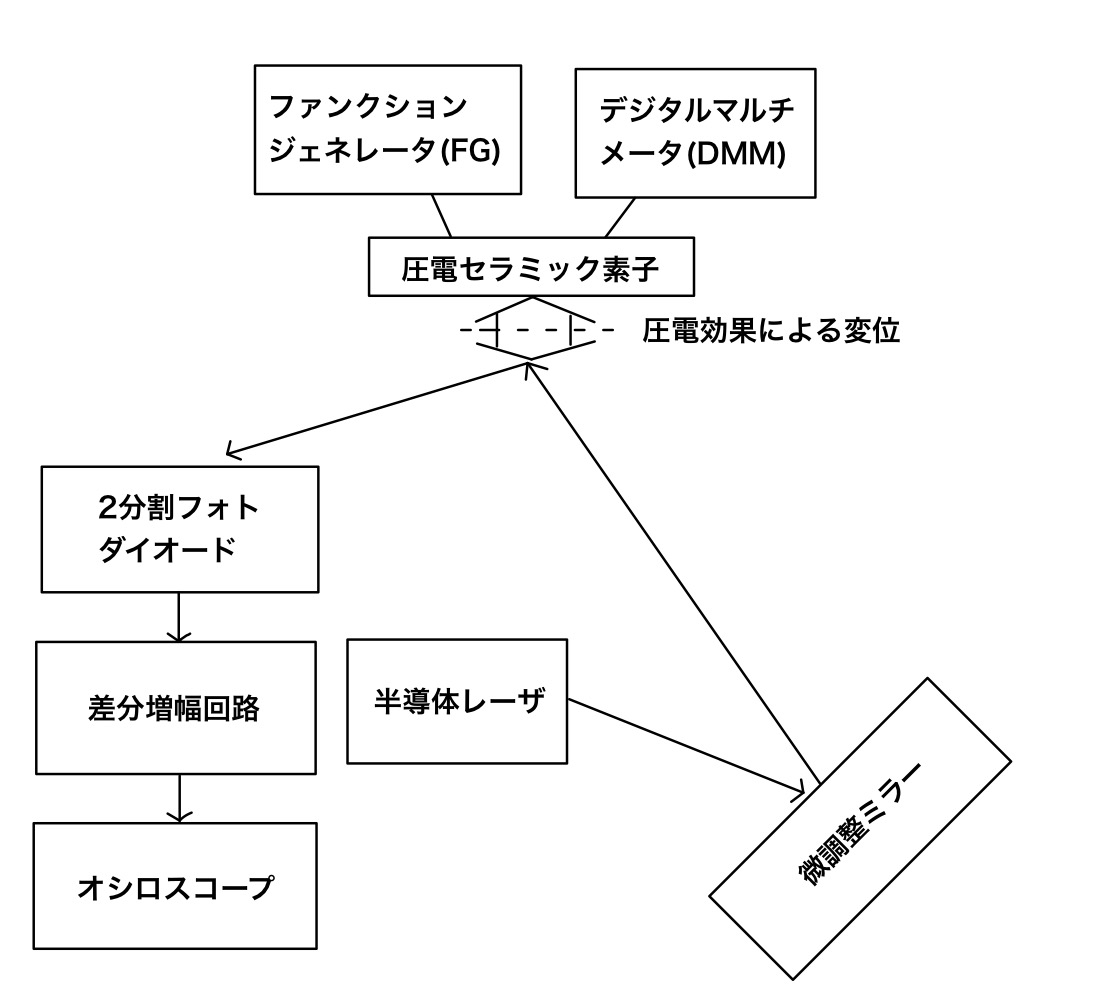
\includegraphics[width = 10cm]{figs/IMG_0321.JPG}
		\caption{圧電セラミック素子への電圧印加による共振現象の測定系ブロック図}
		\label{fig:圧電セラミック素子測定系}
		\end{figure}
		\subsubsection{実験1}
			圧電セラミック素子は,形状の異なる三種類(a:大,b:中,c:小)を用いるが,
			はじめに,圧電セラミック素子aを用いて行った.図\refeq{}に示すように,
			測定システムを構成し,圧電セラミック素子の端子にファンクションジェネレータ
			からの出力を接続した.また,電圧と周波数計測用にデジタルマルチメータの端子
			も接続する.正弦波信号を選択し,周波数は2.0\,kHz~4.0\,kHzの範囲で
			0.1\,kHz程度ごとに変化させた.この時の印加電圧値はデジタルマルチメータ
			によって測定し,3.0\,Vに設定した.次項の実験2,実験3でも同様に3.0\,Vを印加した.

			レーザダイオード(LD)から射出したレーザビームを調整用のミラーの角度を変えながら,
			圧電セラミック素子の金属プレート表面に入射させ,この反射光を2分割フォトダイオード
			のAとBの2つの受光部の中央あたりに入射するように調整ミラー上の調整ネジを回して設定した.
			差分増幅回路のゲイン抵抗($\mathrm{R_G}$)は信号の検出がしやすいようにゲインが大きくなる
			$100\,\Omega 200\,\Omega$ 程度の抵抗値の抵抗値にした.実験1~実験3において,同じゲイン抵抗値を用いた.
			また,出力信号の振幅が最も大きく検出された周波数の波形を記録し,この時の周波数と振幅値の値を測定した.

		\subsubsection{実験2}
			次に,圧電セラミック素子bに素子を変更して実験を行ったが,正弦波信号の周波数は
			4.0\,kHz~6.0\,kHzの範囲で0.1\,kHz程度ごとに変化させた.この時の印加電圧値は,
			3.0\,Vにし,ゲイン抵抗は実験1と同様の値を用いた.また,出力信号の振幅が最も大きく検出された周波数の波形を記録し,
			この時の周波数と振幅値の値を測定した.

		\subsubsection{実験3}
			最後に,圧電セラミック素子cに素子を変更して同様の実験を行ったが,周波数は
			6.0\,kHz~9.0\,kHzの範囲で0.1\,kHz程度ごとに変化させた.この時の印加電圧値は,
			3.0\,Vにし,ゲイン抵抗は実験1と同様の値を用いた.また,出力信号の振幅が最も大きく検出された周波数の波形を記録し,
			この時の周波数と振幅値の値を測定した.

	\subsection{音源の周波数変化による振動状態の光測定}
		\subsubsection{差分増幅回路を用いた光信号検出}
			\subsubsection{実験1:ゲイン抵抗($\mathrm{R_G}$)を変化した場合の出力信号の測定実験}
				
				図に示すような差分増幅回路と光学系を構成し,半導体レーザから出射した
				レーザビームを調整用ミラーの角度を変えながら,音源が入るプラスチックBOX(大)の入口に
				取り付けたミラーに照射した.このミラーから2分割フォトダイオードまでの距離は,15~30\,cmに設定した.
				このミラーから反射されたレーザビームを2分割フォトダイオードのAとBの2つの受光部の中心あたりに入射させた.
				出力波形が明瞭に観察できる光照射位置に調整した.

				差分増幅回路のゲイン抵抗($\mathrm{R_G}$)を調整し,オシロスコープ上に出力波形をモニターした.
				この時,差分増幅回路のゲイン抵抗値をいくつかの値に変化し,音源の周波数設定を変更しながら出力信号波形を
				検出しデータを取得した.

				音源としては,遠隔で操作できるBluetooth対応の小型スピーカーをプラスチック容器に封入し,
				入口にレーザ反射用のミラーを取り付ける.小型スピーカへの信号入力はPC上にインストールされたフリーソフトの
				WabeGeneにより正弦波(sin波)を入力した.出力(音の大きさ)は,PCの音声出力設定で行った.

				\begin{enumerate}
					\item ゲイン抵抗$\mathrm{R_G}$は,オペアンプ(INA103)への電池を外した(電圧OFF)状態で,
						オペアンプの6番ピンと13番ピン間の抵抗値をデジタルマルチメータにより測定する。
						2つの可変抵抗を調整して$\mathrm{R_G}$の値を設定し,周波数を変化した場合の波形をオシロスコープ上で観察し,
						この波形のデータをUSBに記録した.
					\item 実験では,およそ$\mathrm{R_G} = 100\,\Omega, \mathrm{R_G} = 500\,\Omega, \mathrm{R_G} = 1\,\mathrm{k\Omega}$
						のように3段階に設定した.それぞれの$\mathrm{R_G}$設定値において,周波数をPC上で100\,Hz, 150\,Hz, 300\,Hz, 500\,Hz, 1\,kHzまで
						5段階に変化させた。これらの出力波形をオシロスコープ上で検出して波形データを取得した.
					\item 3つの$\mathrm{R_G}$の値のそれぞれに対して取得した波形データから各測定周波数に対する振幅値の値を求める。
						各$\mathrm{R_G}$の値において,横軸:周波数-縦軸:振幅としたグラフを作成し,各自で設定した$\mathrm{R_G}$の測定値と出力電圧との関係を評価した.
				\end{enumerate}

			\subsubsection{実験2:材料の違いによる出力信号測定}
				図\refeq{}に示す即提携において,音源のスピーカーを大小ペアの2つのプラスチックBOXの小さい容器に封入し,これを大きな方のBOXに閉じ込める。
				調整ミラーを用いてスピーカの入るプラスチック容器の表面にレーザビームを照射し,この反射光を2分割フォトダイオード上に入射した.

				差分増幅回路のゲイン抵抗($\mathrm{R_G}$)は100\,\Omega 程度に調整し,周波数をPC上で100\,Hz, 150\,Hz, 300\,Hz, 500\,Hz, 1\,kHzまで
				5段階に変化させた。これらの出力波形をオシロスコープ上で検出して波形データを取得した.

				プラスチック材料からの反射光により求めた測定値を基に横軸:周波数-縦軸:振幅としたグラフを作成し,3.3.2項の実験で作成したグラフを比較して
				プラスチック材質の違いによる出力信号の変化を評価した.

			\subsubsection{実験3:音源から検出器までの距離を変化させた場合の出力信号測定}
				\begin{enumerate}
					\item 図\refeq{}に示す測定系において,音源をプラスチックBOX(大)にスピーカーを入れたものに交換し,表面に反射ミラーを取り付ける。
						このミラーから2分割フォトダイオードまでの距離をおよそ20\,cm, 40\,cm, 60\,cm程度の3段階に変化させた.
						この時,ゲイン抵抗は100\,\Omega 程度に設定した.
					\item 各距離において,周波数をPC上で100\,Hz, 150\,Hz, 300\,Hz, 500\,Hz, 1\,kHzまで5段階に変化させた。
						これらの出力波形をオシロスコープ上で検出して波形データを取得した.
					\item 3段階の距離変化において取得した波形データから各測定周波数に対する振幅値の値を求める。
						各距離において,横軸:周波数-縦軸:振幅としたグラフを作成し,距離と出力電圧との関係を評価する。
				\end{enumerate}
\section{実験結果}
	\subsection{圧電セラミック素子への電圧印加による共振現象の測定}
	\subsection{差分増幅回路を用いた光信号検出}
\section{考察}
	\begin{enumerate}
		\item 2分割フォトダイオードからの出力信号波形を明瞭に得るには,受光部へのレーザビームの照射位置や面積をどのように調整する必要があるか説明する.\\
			光強度が外光よりも十分強くなるように受光部に対して,近距離・小面積で照射する方がレーザ光が散乱せず十分な強度を得ることができる。
			%点光源を考慮した散乱の式
		\item ゲイン抵抗の設定値と出力波形の振幅はどのような関係があるか説明する.\\
			同じ周波数において,ゲイン抵抗を小さくするほど出力信号の振幅は大きくなっている.
			これは,オペアンプを用いた差分増幅回路において,ゲイン抵抗が小さいほど増幅率(ゲイン)が大きくなるため,
			%ゲインの算出式かきます
		\item 音源が入るBOX用の反射材としてミラー板と,プラスチック容器の2種類を比較した.これらの各反射材の厚さを調べ,物理的形状の違いが出力波形にどのように影響しているか説明する.\\
			ミラー板の厚さは575\,μm,プラスチック容器の厚さ2014\,μmであった.実験1と実験2のゲイン抵抗100\,\Omega の場合の出力値を比較すると,ミラー板の方は100~300\,Hzまでは周波数に比例して振幅値が上昇していることがわかる.
			次に,プラスチック容器の場合は周波数が増えるにつれ,指数関数的に減衰していることがわかる.また,周波数ごとの振幅を比較すると,測定した全ての周波数において
			ミラー板の方がプラスチック容器よりも振幅が大きくなっていることが読み取れる.

			したがって,反射材の厚さに反比例して振幅が変化するように影響しているとわかる.
		\item 音源の周波数の設定値によっては出力波形に入力信号と異なる周波数が重畳したり,ひずみやノイズが生じたりする場合があるが,これらの現象にはどのような要因が影響していると考えられるか.\\
			出力波形の歪みについて,波形全体が60Hz程度で振動していた.これは,測定場所の照明が外乱として入力信号に加えられていると考えられる。
			特に,周波数が高くなると出力波形の線が太くなった(ノイズが発生した)ため,同じ外乱成分でも周波数が高くなるにつれ,振幅が低下してS/N比が低くなってしまい,
			外乱成分が出力波形に顕著に現れてしまうためだと考えられる。
	\end{enumerate}
\begin{thebibliography}{99}
\bibitem{ref:圧電効果}
	TDK「身の回りにある圧電効果」閲覧日 2023/12/26\\
	https://www.tdk.com/ja/tech-mag/knowledge/089
\end{thebibliography}
\end{document}